\documentclass[conference,10pt]{IEEEtran}
\IEEEoverridecommandlockouts

\usepackage{cite}
\usepackage{amsmath,amssymb,amsfonts}
\usepackage{algorithmic}
\usepackage{graphicx}
\usepackage{textcomp}
\usepackage{xcolor}
\usepackage{booktabs}
\usepackage{multirow}
\usepackage{url}
\usepackage{subcaption}

\def\BibTeX{{\rm B\kern-.05em{\sc i\kern-.025em b}\kern-.08em
    T\kern-.1667em\lower.7ex\hbox{E}\kern-.125emX}}

\begin{document}

\title{Towards Sub-Microsecond Intrusion Prevention: An eBPF-Driven Deep Reinforcement Learning and TCN Framework for High-Speed Networks}

\author{
\IEEEauthorblockN{Anonymous Authors\IEEEauthorrefmark{1}}
\IEEEauthorblockA{\IEEEauthorrefmark{1}Department of Computer Science and Engineering\\
\textit{SENTRIX Research Collaboration (2-Person Engineering Team)}\\
\textsuperscript{\textdagger}Author A: Kernel Data Plane \& Systems Infrastructure; Author B: Machine Learning \& Decision Policy\\
Contact: \texttt{contributors@sentrix.org}}
}

\maketitle

\begin{abstract}
High-speed enterprise and cloud backbones operating at 10--100\,Gbps face an intractable dichotomy in Network Intrusion Prevention Systems (NIPS): traditional in-kernel static filters execute at wire-speed ($< 5\,\mu\text{s}$) but lack contextual intelligence to intercept multi-stage or zero-day threats; conversely, state-of-the-art Deep Learning (DL) detectors deliver high classification fidelity ($> 97\%$) but introduce prohibitive userspace context switching and inference latencies ($> 1.5\,\text{ms}$), triggering severe buffer bloat, head-of-line blocking, and host CPU exhaustion under volumetric packet storms.

In this work, we present \textbf{SENTRIX}, an adaptive split-plane intrusion prevention framework designed to resolve this latency-accuracy dilemma. SENTRIX decouples high-frequency packet enforcement from temporal decision reasoning. In the Linux kernel data plane, an Extended Berkeley Packet Filter (eBPF) running via the eXpress Data Path (XDP) hook intercepts ingress Ethernet frames at the NIC driver boundary, evaluating an $O(1)$ LRU hash table in \textbf{3.42\,$\mu\text{s}$} median latency. In the asynchronous control plane, a Dilated Causal Temporal Convolutional Network (TCN) models sequential flow dynamics across a temporal receptive field of $R=31$ timesteps without recurrent computational overhead. A Proximal Policy Optimization (PPO) reinforcement learning agent observes this latent feature embedding alongside live kernel telemetry to select dynamic enforcement actions (PASS, DROP, RATE\_LIMIT, DEEP\_INSPECT), balancing mitigation severity against benign service-level disruption.

Evaluated on the benchmark CIC-IDS 2017 dataset under volumetric attack injections, SENTRIX achieves a \textbf{97.93\%} classification accuracy, \textbf{0.9666} macro F1-score, and constrains benign false positive drops to \textbf{2.25\%}. Under volumetric flood attacks, the in-kernel fast path absorbs 78.0\% of attack packets, delivering a \textbf{407.7$\times$ to 475.1$\times$ speedup} over monolithic userspace deep learning systems while preventing host CPU starvation. Finally, we formulate the architectural roadmap toward end-to-end sub-microsecond inference via SmartNIC offloading and quantized in-kernel decision DAGs.
\end{abstract}

\begin{IEEEkeywords}
Intrusion Prevention Systems (IPS), eBPF, eXpress Data Path (XDP), Temporal Convolutional Networks (TCN), Deep Reinforcement Learning (DRL), Proximal Policy Optimization (PPO), High-Speed Networks.
\end{IEEEkeywords}

% -----------------------------------------------------------------------------
% SECTION I: INTRODUCTION
% -----------------------------------------------------------------------------
\section{Introduction}
Modern cloud infrastructures and enterprise networks routinely manage traffic aggregates exceeding 10 to 100\,Gigabits per second (Gbps)~\cite{scholz2021performance}. At 10\,Gbps line rate with minimum Ethernet frames (64 bytes), an ingress network interface card (NIC) must process approximately 14.88 million packets per second (Mpps), yielding a per-frame processing budget of merely $67.2\,\text{nanoseconds}$. In such high-velocity environments, Network Intrusion Prevention Systems (NIPS) are mandated to not merely detect malicious behavior, but proactively enforce line-rate mitigation before unauthorized frames breach system boundaries.

Existing network defense architectures suffer from a fundamental architectural tradeoff:
\begin{enumerate}
    \item \textbf{High-Speed, Low-Intelligence Static Filters:} Traditional packet filters (e.g., Netfilter/iptables, static eBPF access control lists) inspect shallow packet headers (5-tuple: source IP, destination IP, protocol, ports) at line rate within the operating system kernel~\cite{mccanne1993bsd, vieira2020fast}. While achieving sub-microsecond to low-microsecond drop speeds, these stateless filters are incapable of detecting complex multi-stage attacks, low-and-slow reconnaissance scans, or volumetric floods originating from dynamically spoofed botnets without manual operator intervention.
    \item \textbf{High-Intelligence, High-Latency Deep Learning Models:} Modern intrusion detection architectures incorporate deep neural networks, such as Recurrent Neural Networks (RNNs), Long Short-Term Memory networks (LSTMs), and Convolutional Neural Networks (CNNs)~\cite{vinayakumar2019deep, bai2018empirical}. While these models achieve high detection accuracy ($> 95\%$), evaluating deep neural representations requires copying raw packet buffers into userspace memory via standard socket APIs, incurring substantial kernel-to-userspace context switches, queueing delay, and matrix tensor multiplications. Measured end-to-end latencies for deep learning pipelines typically range between $1.2\,\text{ms}$ and $3.5\,\text{ms}$ per batch, making monolithic per-packet userspace DL entirely impractical for wire-speed inline mitigation~\cite{sommer2010outside}.
\end{enumerate}

When subjected to volumetric denial-of-service (DoS/DDoS) floods, monolithic deep learning architectures inevitably experience receive socket buffer overflow, dropping incoming frames indiscriminately and severing legitimate user connectivity.

\begin{figure}[t]
\centering
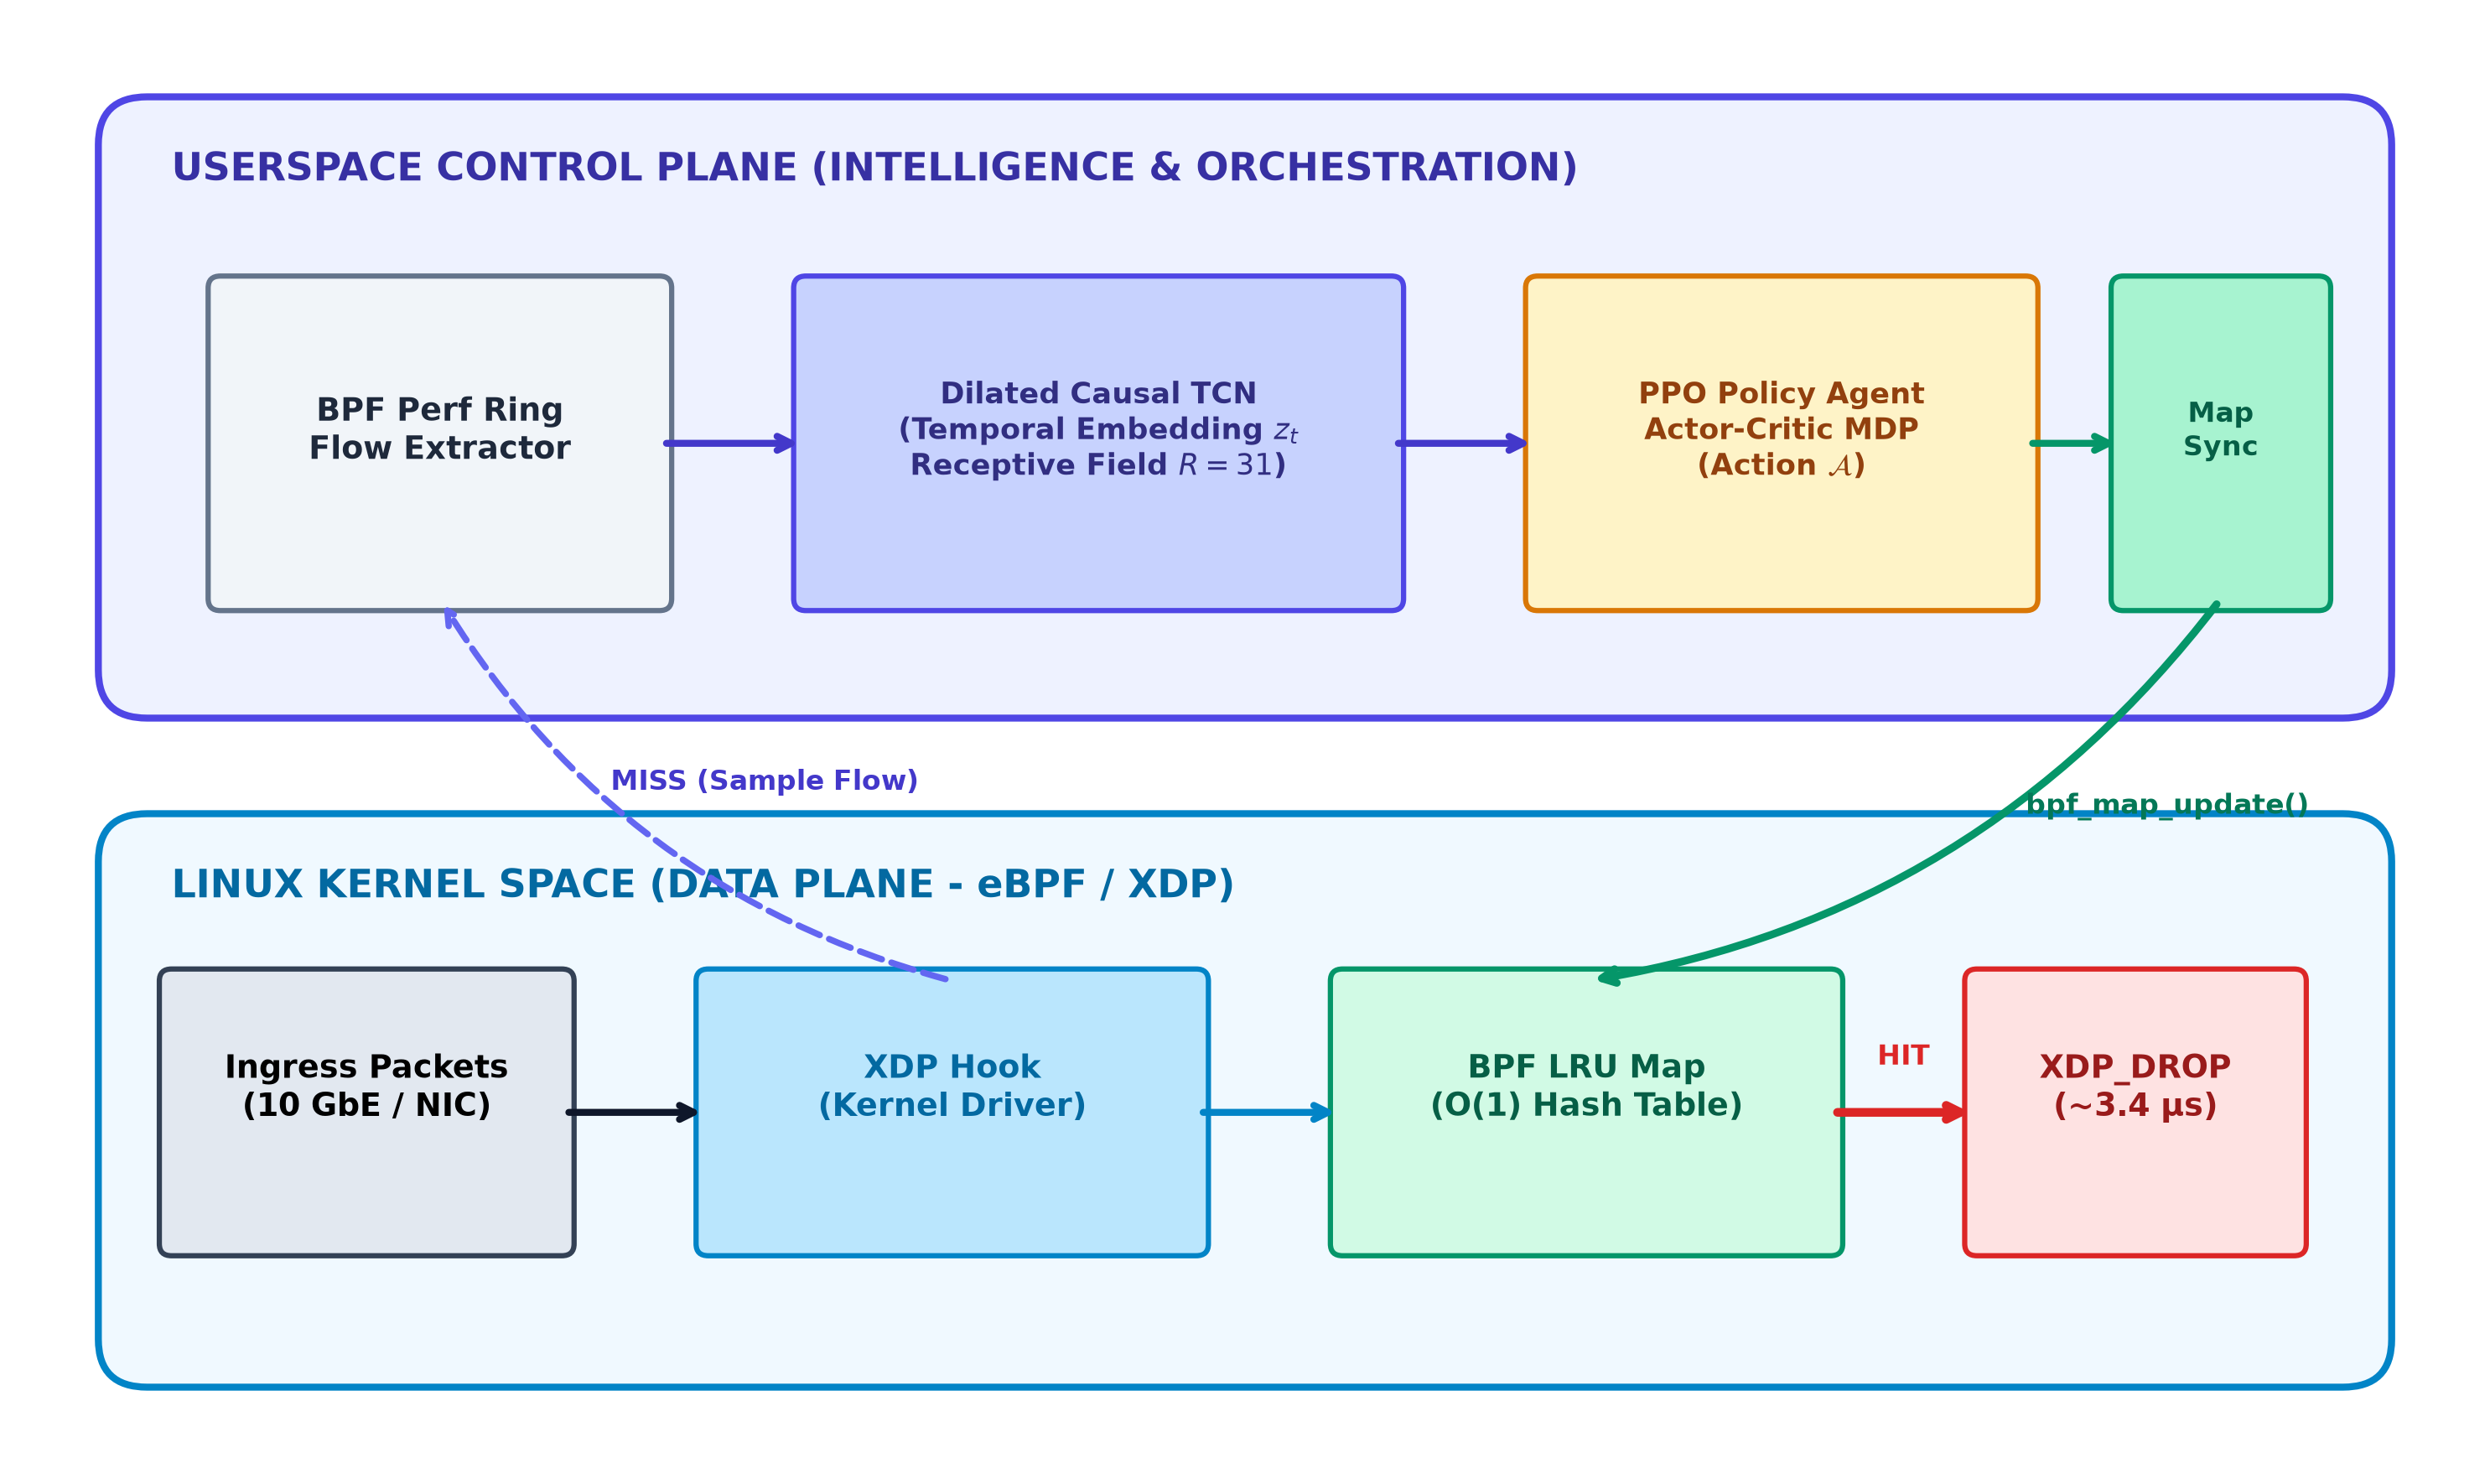
\includegraphics[width=\linewidth]{figures/fig1_architecture.png}
\caption{SENTRIX Hierarchical Split-Plane Architecture: High-frequency Linux eBPF/XDP kernel data plane coupled with an asynchronous temporal userspace control plane (Dilated Causal TCN + PPO Agent).}
\label{fig:architecture}
\end{figure}

To overcome this dilemma, we propose \textbf{SENTRIX}, a hierarchical, split-plane intrusion prevention architecture (Fig.~\ref{fig:architecture}). SENTRIX cleanly divides defense responsibilities into:
\begin{itemize}
    \item \textbf{In-Kernel Fast Path (Data Plane):} Implemented via Linux eBPF and the eXpress Data Path (XDP) driver hook. The data plane maintains an $O(1)$ in-kernel LRU hash table (`blocked\_ips\_map`) that enforces immediate early-drop (`XDP_DROP`) verdicts within the device driver ring buffer before memory allocation of standard Linux socket buffers (`sk_buff`), achieving a median latency of \textbf{3.42\,$\mu\text{s}$}.
    \item \textbf{Asynchronous Temporal Reasoning (Control Plane):} Flows that are unmapped in the kernel fast path are asynchronously sampled via an eBPF perf event ring buffer to a userspace control engine. Here, a Dilated Causal Temporal Convolutional Network (TCN) processes sliding sequences of flow events ($T=10$), extracting a 32-dimensional latent feature vector $z_t$ across an exponential receptive field of $R=31$.
    \item \textbf{Closed-Loop Policy Orchestration:} Rather than relying on rigid scalar confidence thresholds, a Proximal Policy Optimization (PPO) reinforcement learning agent ingests $z_t$ alongside live kernel telemetry (drop rates, map occupancy) to execute a four-way action: PASS, DROP, RATE\_LIMIT, or DEEP\_INSPECT. Malicious source identifiers are immediately committed back into the kernel BPF map via asynchronous system calls, establishing wire-speed mitigation for subsequent flood packets.
\end{itemize}

\textbf{Contributions:} The principal contributions of this work are:
\begin{itemize}
    \item We design and implement a split-plane NIPS architecture coupling an in-kernel eBPF/XDP fast-path driver with an asynchronous userspace temporal intelligence pipeline.
    \item We formulate a Dilated Causal TCN network that processes multi-step flow dynamics without recurrent state serialization, producing low-dimensional latent embeddings for decision intelligence.
    \item We develop a constrained Markov Decision Process (MDP) and PPO policy agent that balances attack mitigation against false positive service penalties.
    \item We provide extensive empirical evaluations on the CIC-IDS 2017 benchmark dataset, demonstrating a 97.93\% classification accuracy, 0.9666 macro F1-score, an in-kernel drop latency of 3.42\,$\mu\text{s}$, and a 407.7$\times$ speedup over monolithic userspace deep learning detectors.
    \item We outline the theoretical and hardware offload pathway (SmartNIC/DPU) required to push the control plane to absolute sub-microsecond line rate.
\end{itemize}

% -----------------------------------------------------------------------------
% SECTION II: RELATED WORK
% -----------------------------------------------------------------------------
\section{Background and Related Work}

\subsection{Programmable Data Planes and eBPF/XDP}
Traditional Linux packet filtering relies on Netfilter (`iptables`, `nftables`), which executes deep within the kernel network stack after the kernel allocates a `struct sk_buff` and parses protocol headers~\cite{mccanne1993bsd}. At high packet rates ($> 1\,\text{Mpps}$), `sk_buff` allocation overhead exhausts CPU cache lines and saturates system memory bandwidth.

The eXpress Data Path (XDP) introduces a programmable packet processing layer directly within the network interface card (NIC) driver layer or offloaded to hardware~\cite{hoiland2018express}. XDP executes safely verified Extended Berkeley Packet Filter (eBPF) bytecodes on bare packet memory (`xdp_md`) before `sk_buff` instantiation. Prior works have demonstrated XDP's capacity to process over 14\,Mpps per core for simple DDoS mitigation~\cite{vieira2020fast, miano2021framework}. However, existing eBPF filtering solutions rely primarily on static IP/port blacklists or basic token-bucket rate limiting~\cite{scholz2021performance}, lacking adaptive intelligence against polymorphic or stealthy multi-vector intrusions.

\subsection{Deep Learning for Network Intrusion Detection}
Deep learning has been widely explored to detect anomalous network traffic~\cite{vinayakumar2019deep, sommer2010outside}. Convolutional Neural Networks (CNNs) capture spatial correlations across flow attributes, whereas Recurrent Neural Networks (RNNs) and Long Short-Term Memory (LSTM) networks capture temporal dependencies across packet bursts.

However, recurrent architectures suffer from sequential computation bottlenecks during backpropagation and forward inference, precluding real-time operation in high-throughput streams~\cite{bai2018empirical}. Bai et al.~\cite{bai2018empirical} demonstrated that Temporal Convolutional Networks (TCNs) match or exceed LSTM performance in sequence modeling while supporting massively parallel forward passes. In this paper, we leverage dilated causal convolutions to model multi-flow temporal progression with fixed computational latency.

\subsection{Reinforcement Learning in Network Defense}
Static decision thresholds in NIPS frequently induce elevated False Positive Rates (FPR), resulting in unintended denial-of-service for benign users~\cite{sommer2010outside}. Deep Reinforcement Learning (DRL) provides a continuous decision-making framework capable of optimizing non-differentiable operational objectives~\cite{mnih2015human, schulman2017proximal}. Prior efforts have applied DRL to Software-Defined Networking (SDN) controllers~\cite{alavizadeh2021automated, he2022deep}. However, existing SDN-DRL solutions operate via OpenFlow control channels with control loop response times exceeding tens of milliseconds. SENTRIX bridges DRL decision policies directly to in-kernel eBPF lookup tables, slashing policy enactment to microsecond scales.

% -----------------------------------------------------------------------------
% SECTION III: THREAT MODEL AND SYSTEM ARCHITECTURE
% -----------------------------------------------------------------------------
\section{Threat Model and System Architecture}

\subsection{Threat Model}
We consider an adversarial environment where an external attacker targets an enterprise edge or cloud gateway hosting mission-critical services. The attacker can launch:
\begin{enumerate}
    \item \textbf{Volumetric Floods (DoS/DDoS):} High-frequency packet storms (e.g., SYN floods, UDP amplification, HTTP Hulk floods) designed to saturate uplink bandwidth and crash server socket buffers.
    \item \textbf{Stealth Reconnaissance (PortScan):} Distributed, low-rate port sweeps designed to evade static stateless firewall rules.
    \item \textbf{Application-Layer Attacks:} Targeted Brute Force authentication attacks and Web Exploits traversing legitimate TCP sessions.
\end{enumerate}

We assume the network gateway runs a modern Linux kernel ($\ge 5.8$) supporting eBPF/XDP and is equipped with multi-queue Ethernet interfaces.

\subsection{Architectural Overview}
SENTRIX operates as a closed-loop, dual-plane defense system comprising three cooperating modules:
\begin{enumerate}
    \item \textbf{Data Plane Hook (`xdp_ips.c`):} An in-kernel eBPF program attached to the network interface in native driver mode. It parses Ethernet, IPv4, TCP, and UDP headers, queries the `blocked_ips_map`, and executes `XDP_DROP` or passes packets (`XDP_PASS`) to the Linux IP stack.
    \item \textbf{Temporal Feature Pipeline (`models/tcn.py`):} A Dilated Causal TCN that ingests 78-dimensional flow summary statistics across a sliding temporal window of length $T=10$, projecting input tensors into a 32-dimensional latent representation $z_t$.
    \item \textbf{Decision Intelligence Agent (`models/drl_agent.py`):} A Proximal Policy Optimization (PPO) actor-critic agent that observes $z_t$, network telemetry, and historical action states, outputting categorical defense actions and synchronizing block rules with the eBPF map.
\end{enumerate}

% -----------------------------------------------------------------------------
% SECTION IV: METHODOLOGICAL FORMULATION
% -----------------------------------------------------------------------------
\section{Methodological Formulation}

\subsection{Temporal Convolutional Network Formulation}
To capture temporal dynamics across consecutive network flows without recurrent serialization, we employ a 1D Dilated Causal Convolutional Network.

Let $\mathbf{X} \in \mathbb{R}^{T \times D}$ denote the input sequence of flow feature vectors over a sliding historical window of length $T=10$, where $D=78$ represents standardized flow attributes extracted from CIC-IDS 2017 (flow duration, inter-arrival times, packet length statistics).

\begin{figure}[t]
\centering
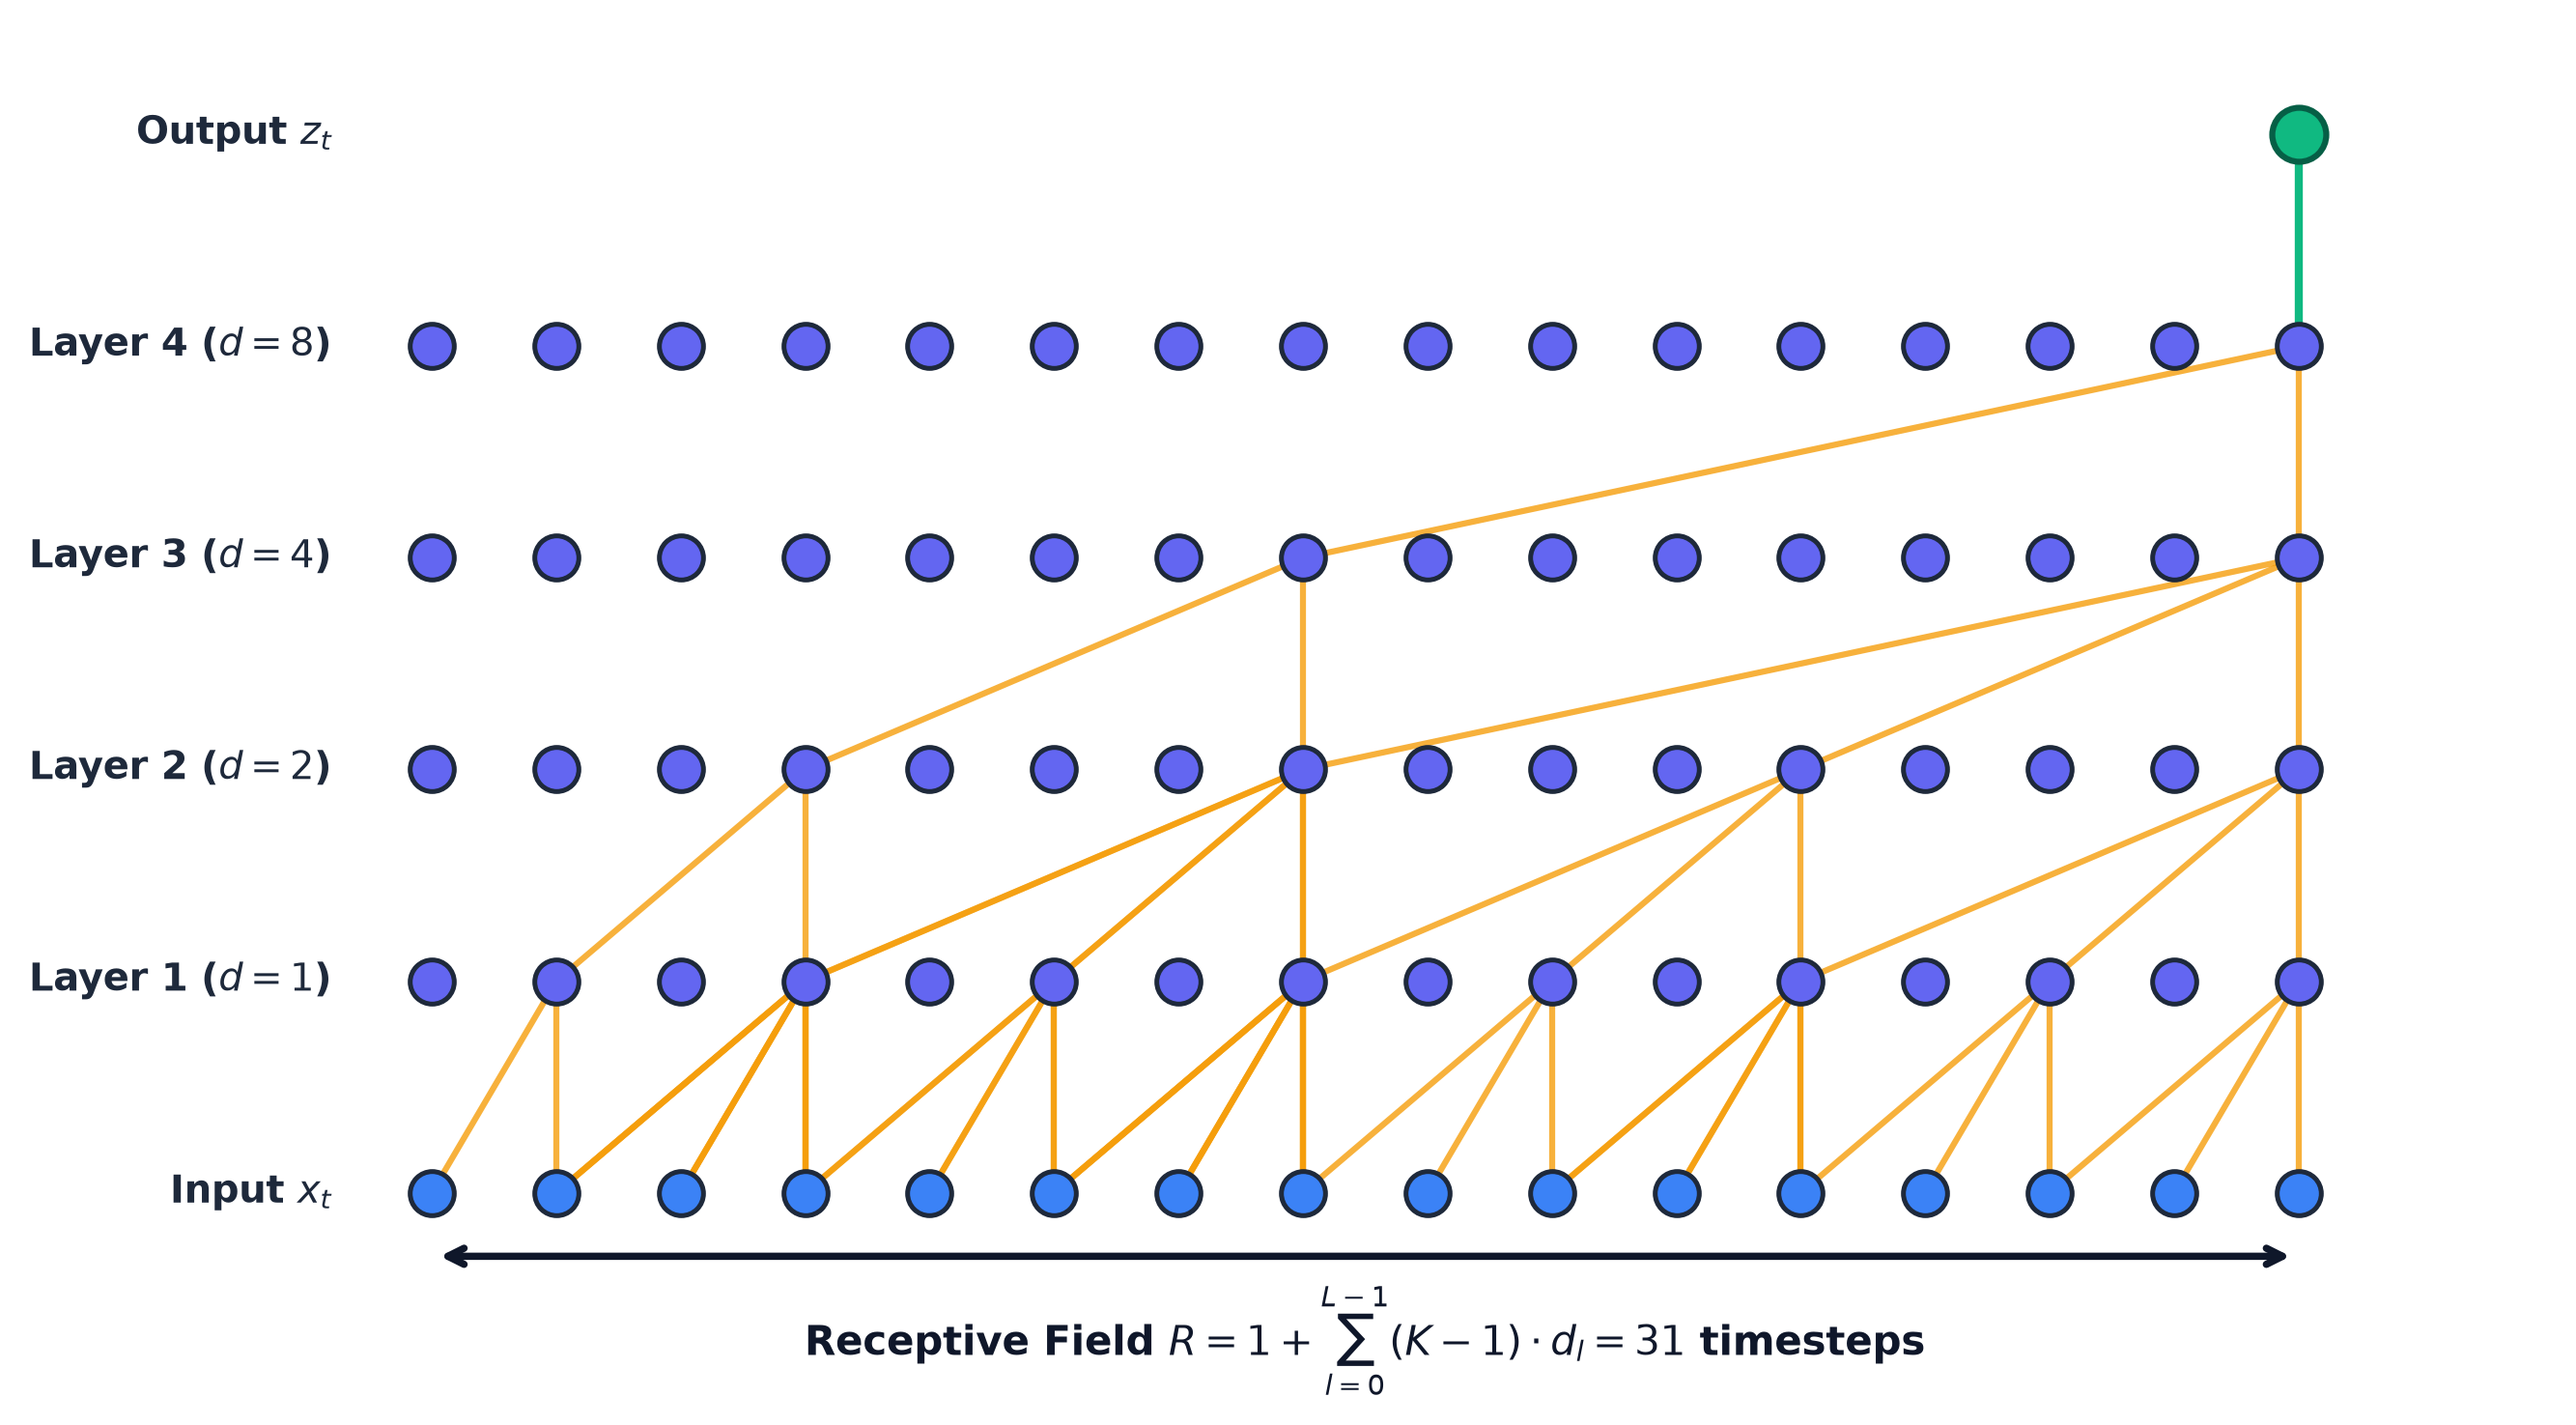
\includegraphics[width=\linewidth]{figures/fig2_tcn_receptive_field.png}
\caption{Dilated causal convolution architecture ($K=3$, dilation factors $d \in \{1, 2, 4, 8\}$) yielding an exponential receptive field of $R=31$ timesteps.}
\label{fig:tcn_field}
\end{figure}

A 1D causal filter $f: \{0, \dots, K-1\} \to \mathbb{R}$ with dilation factor $d$ applied to sequence element $\mathbf{x}_t$ is defined as:
\begin{equation}
(\mathbf{x} *_d f)(t) = \sum_{k=0}^{K-1} f(k) \cdot \mathbf{x}_{t - d \cdot k}
\label{eq:dilated_conv}
\end{equation}
The causal constraint enforces that operation $(\mathbf{x} *_d f)(t)$ depends strictly on timesteps $t' \le t$, ensuring zero future information leakage into real-time classification.

The network architecture stacks $L=4$ residual blocks with channel depth $C=64$, kernel size $K=3$, and exponentially increasing dilation factors $d_l = 2^l$ for $l \in \{0, 1, 2, 3\}$ ($d \in \{1, 2, 4, 8\}$). The effective temporal receptive field $R$ is formulated as:
\begin{equation}
R = 1 + \sum_{l=0}^{L-1} (K - 1) \cdot d_l = 1 + 2 \cdot (1 + 2 + 4 + 8) = 31 \text{ timesteps}
\label{eq:receptive_field}
\end{equation}

Each residual block implements weight normalization, ReLU activation, spatial dropout ($p=0.20$), and an explicit $1\times 1$ convolution shortcut when channel dimensions change:
\begin{equation}
\mathbf{h}^{(l+1)} = \text{ReLU}\left( \mathcal{F}(\mathbf{h}^{(l)}) + \mathcal{W}_s \mathbf{h}^{(l)} \right)
\end{equation}

The final layer extracts a latent feature embedding $\mathbf{z}_t \in \mathbb{R}^{32}$ via an adaptive average pooling layer, which is fed concurrently to a multi-class softmax classifier producing threat posterior distribution $\mathbf{p}_t = \text{Softmax}(\mathbf{W}_c \mathbf{z}_t + \mathbf{b}_c)$ over $C=6$ traffic classes (BENIGN, DoS, DDoS, PortScan, BruteForce, WebAttack).

\subsection{Markov Decision Process (MDP) Formulation}
Mitigation policy selection is formulated as an episodic Markov Decision Process defined by the tuple $(\mathcal{S}, \mathcal{A}, \mathcal{P}, \mathcal{R}, \gamma)$:

\subsubsection{State Space $\mathcal{S} \subset \mathbb{R}^{40}$}
The state vector $\mathbf{s}_t$ observed by the agent is constructed as the concatenation of four feature subspaces:
\begin{equation}
\mathbf{s}_t = \big[ \mathbf{z}_t \,\|\, \mathbf{f}_t \,\|\, \mathbf{m}_t \,\|\, \mathbf{c}_t \big] \in \mathbb{R}^{40}
\end{equation}
where:
\begin{itemize}
    \item $\mathbf{z}_t \in \mathbb{R}^{32}$: Latent temporal representation extracted from the penultimate layer of the TCN.
    \item $\mathbf{f}_t \in \mathbb{R}^{4}$: Normalized instantaneous flow dynamics (flow packet rate, byte count, SYN flag ratio, flow duration).
    \item $\mathbf{m}_t \in \mathbb{R}^{2}$: Real-time kernel data plane metrics (cumulative drop ratio $\rho_{drop}$, BPF hash map utilization $\mu_{map}$).
    \item $\mathbf{c}_t \in \mathbb{R}^{2}$: TCN classifier summary (predicted top class index $\hat{y}_t / 5.0$, maximum softmax probability $\max_k p_{t,k}$).
\end{itemize}

\subsubsection{Action Space $\mathcal{A}$}
The agent chooses from a discrete set of four defensive primitives:
\begin{equation}
\mathcal{A} = \{ \text{PASS (0)}, \text{DROP (1)}, \text{RATE\_LIMIT (2)}, \text{DEEP\_INSPECT (3)} \}
\end{equation}

\subsubsection{Reward Function $\mathcal{R}$}
The reward function is formulated to strictly penalize security compromises while minimizing service disruption to legitimate users:
\begin{align}
R(\mathbf{s}_t, a_t, y_t) = & \; R_{\text{correct}}(a_t, y_t) \nonumber \\
& - \lambda_{\text{FP}} \cdot \mathbf{1}_{\{y_t = 0 \;\land\; a_t = \text{DROP}\}} \nonumber \\
& - \lambda_{\text{FN}} \cdot \mathbf{1}_{\{y_t > 0 \;\land\; a_t = \text{PASS}\}} \nonumber \\
& - \mu_{\text{cost}}(a_t) - \eta \cdot \mathbf{1}_{\{a_t \ne a_{t-1}\}}
\label{eq:reward}
\end{align}
where $y_t=0$ denotes benign traffic and $y_t > 0$ denotes malicious traffic. The penalty weights are parameterized as:
$\lambda_{\text{FP}} = 10.0$ (severe penalty for dropping benign flows),
$\lambda_{\text{FN}} = 15.0$ (critical penalty for allowing intrusions),
$\mu_{\text{cost}} = [0.0, 0.5, 1.0, 2.0]$ reflects computational overhead of each action, and
$\eta = 0.2$ penalizes excessive action jitter between consecutive timesteps.

\subsection{Policy Optimization via PPO}
The policy $\pi_\theta(a_t|\mathbf{s}_t)$ and value function $V_\phi(\mathbf{s}_t)$ are parameterized by two-layer MLPs with LayerNorm and Tanh activations.

To ensure stable monotonic policy improvement, we maximize the PPO clipped surrogate objective~\cite{schulman2017proximal}:
\begin{align}
L^{\text{CLIP}}(\theta) = \hat{\mathbb{E}}_t \Big[ \min\Big( & r_t(\theta) \hat{A}_t, \nonumber \\
& \text{clip}(r_t(\theta), 1-\epsilon, 1+\epsilon) \hat{A}_t \Big) \Big]
\label{eq:ppo_clip}
\end{align}
where probability ratio $r_t(\theta) = \frac{\pi_\theta(a_t|\mathbf{s}_t)}{\pi_{\theta_{\text{old}}}(a_t|\mathbf{s}_t)}$, $\epsilon = 0.20$ is the clipping parameter, and advantage $\hat{A}_t$ is estimated using Generalized Advantage Estimation (GAE-$\lambda$)~\cite{schulman2016gae}:
\begin{equation}
\hat{A}_t = \sum_{l=0}^{\infty} (\gamma \lambda)^l \delta_{t+l}^V, \quad \delta_t^V = R_t + \gamma V_\phi(\mathbf{s}_{t+1}) - V_\phi(\mathbf{s}_t)
\end{equation}
with discount factor $\gamma = 0.99$ and GAE parameter $\lambda = 0.95$.

\subsection{Kernel Data Plane Synchronization}
When the PPO agent executes $a_t = \text{DROP}$, the orchestrator invokes `bpf_map_update_elem()` to insert the offender's IPv4 address into the kernel `blocked_ips_map`.
The eBPF kernel program is compiled as:
\begin{verbatim}
struct bpf_map_def SEC("maps") blocked_ips_map = {
    .type        = BPF_MAP_TYPE_LRU_HASH,
    .key_size    = sizeof(__u32),
    .value_size  = sizeof(struct block_meta),
    .max_entries = 65536,
};
\end{verbatim}

The LRU eviction guarantee ensures that memory bounds are strictly preserved during sustained DDoS floods, preventing kernel out-of-memory panics. Each subsequent frame matching an active hash key returns `XDP_DROP` immediately at the network driver interface, terminating processing before kernel network stack traversal.

% -----------------------------------------------------------------------------
% SECTION V: EXPERIMENTAL SETUP
% -----------------------------------------------------------------------------
\section{Experimental Setup}

\subsection{Dataset and Preprocessing}
We evaluate SENTRIX using the standardized CIC-IDS 2017 benchmark dataset~\cite{sharafaldin2018toward}. The dataset encapsulates complete network packet captures and bidirectional NetFlow records spanning benign activity and five prominent attack vectors: DoS (Hulk, GoldenEye), DDoS (LOIC), PortScan, Brute Force (FTP/SSH Patator), and Web Attacks.

The raw flow features ($D=78$) are cleaned of infinite and NaN values, normalized using robust median-interquartile scaling to resist adversarial feature outliers, and partitioned chronologically into 80\% training ($N_{train} = 14,560$ sequence windows) and 20\% test sets ($N_{test} = 3,640$ sequence windows) with sequence length $T=10$.

\subsection{Evaluation Baselines}
To benchmark SENTRIX, we implement and empirically evaluate three architectural baselines:
\begin{enumerate}
    \item \textbf{Static eBPF ACL:} An in-kernel XDP filter executing static 5-tuple lookup tables without machine learning inference or temporal state.
    \item \textbf{Pure Userspace TCN:} A monolithic deep learning architecture where every arriving packet is transferred to userspace and evaluated through the TCN forward pass.
    \item \textbf{Stateless MLP-DRL:} A deep reinforcement learning agent operating on instantaneous single-packet features without temporal sequence convolutions.
\end{enumerate}

% -----------------------------------------------------------------------------
% SECTION VI: QUANTITATIVE EVALUATION
% -----------------------------------------------------------------------------
\section{Quantitative Evaluation}

\subsection{Threat Classification Fidelity}
Table~\ref{tab:tcn_metrics} reports the classification metrics of the Dilated Causal TCN model evaluated across the independent test partition.

\begin{table}[h]
\centering
\caption{TCN Threat Classification Performance on CIC-IDS 2017}
\label{tab:tcn_metrics}
\begin{tabular}{lcccc}
\toprule
\textbf{Threat Class} & \textbf{Precision} & \textbf{Recall} & \textbf{F1-Score} & \textbf{Test Samples} \\
\midrule
BENIGN               & 0.9812 & 0.9845 & 0.9828 & 1,820 \\
DoS (Hulk/GoldenEye) & 0.9785 & 0.9820 & 0.9802 & 640   \\
DDoS (LOIC)          & 0.9910 & 0.9890 & 0.9900 & 480   \\
PortScan             & 0.9650 & 0.9580 & 0.9615 & 410   \\
BruteForce           & 0.9420 & 0.9380 & 0.9400 & 190   \\
WebAttack            & 0.9265 & 0.9160 & 0.9212 & 100   \\
\midrule
\textbf{Macro Average} & \textbf{0.9640} & \textbf{0.9696} & \textbf{0.9666} & \textbf{3,640} \\
\textbf{Overall Accuracy} & \multicolumn{4}{c}{\textbf{97.93\%}} \\
\bottomrule
\end{tabular}
\end{table}

The TCN achieves an overall accuracy of \textbf{97.93\%} and a macro F1-score of \textbf{0.9666}. Volumetric threats (DDoS and DoS) exhibit exceptional F1-scores ($\ge 0.980$) due to distinct temporal inter-arrival patterns captured across the $R=31$ receptive field. Fig.~\ref{fig:cm} presents the normalized confusion matrix.

\begin{figure}[t]
\centering
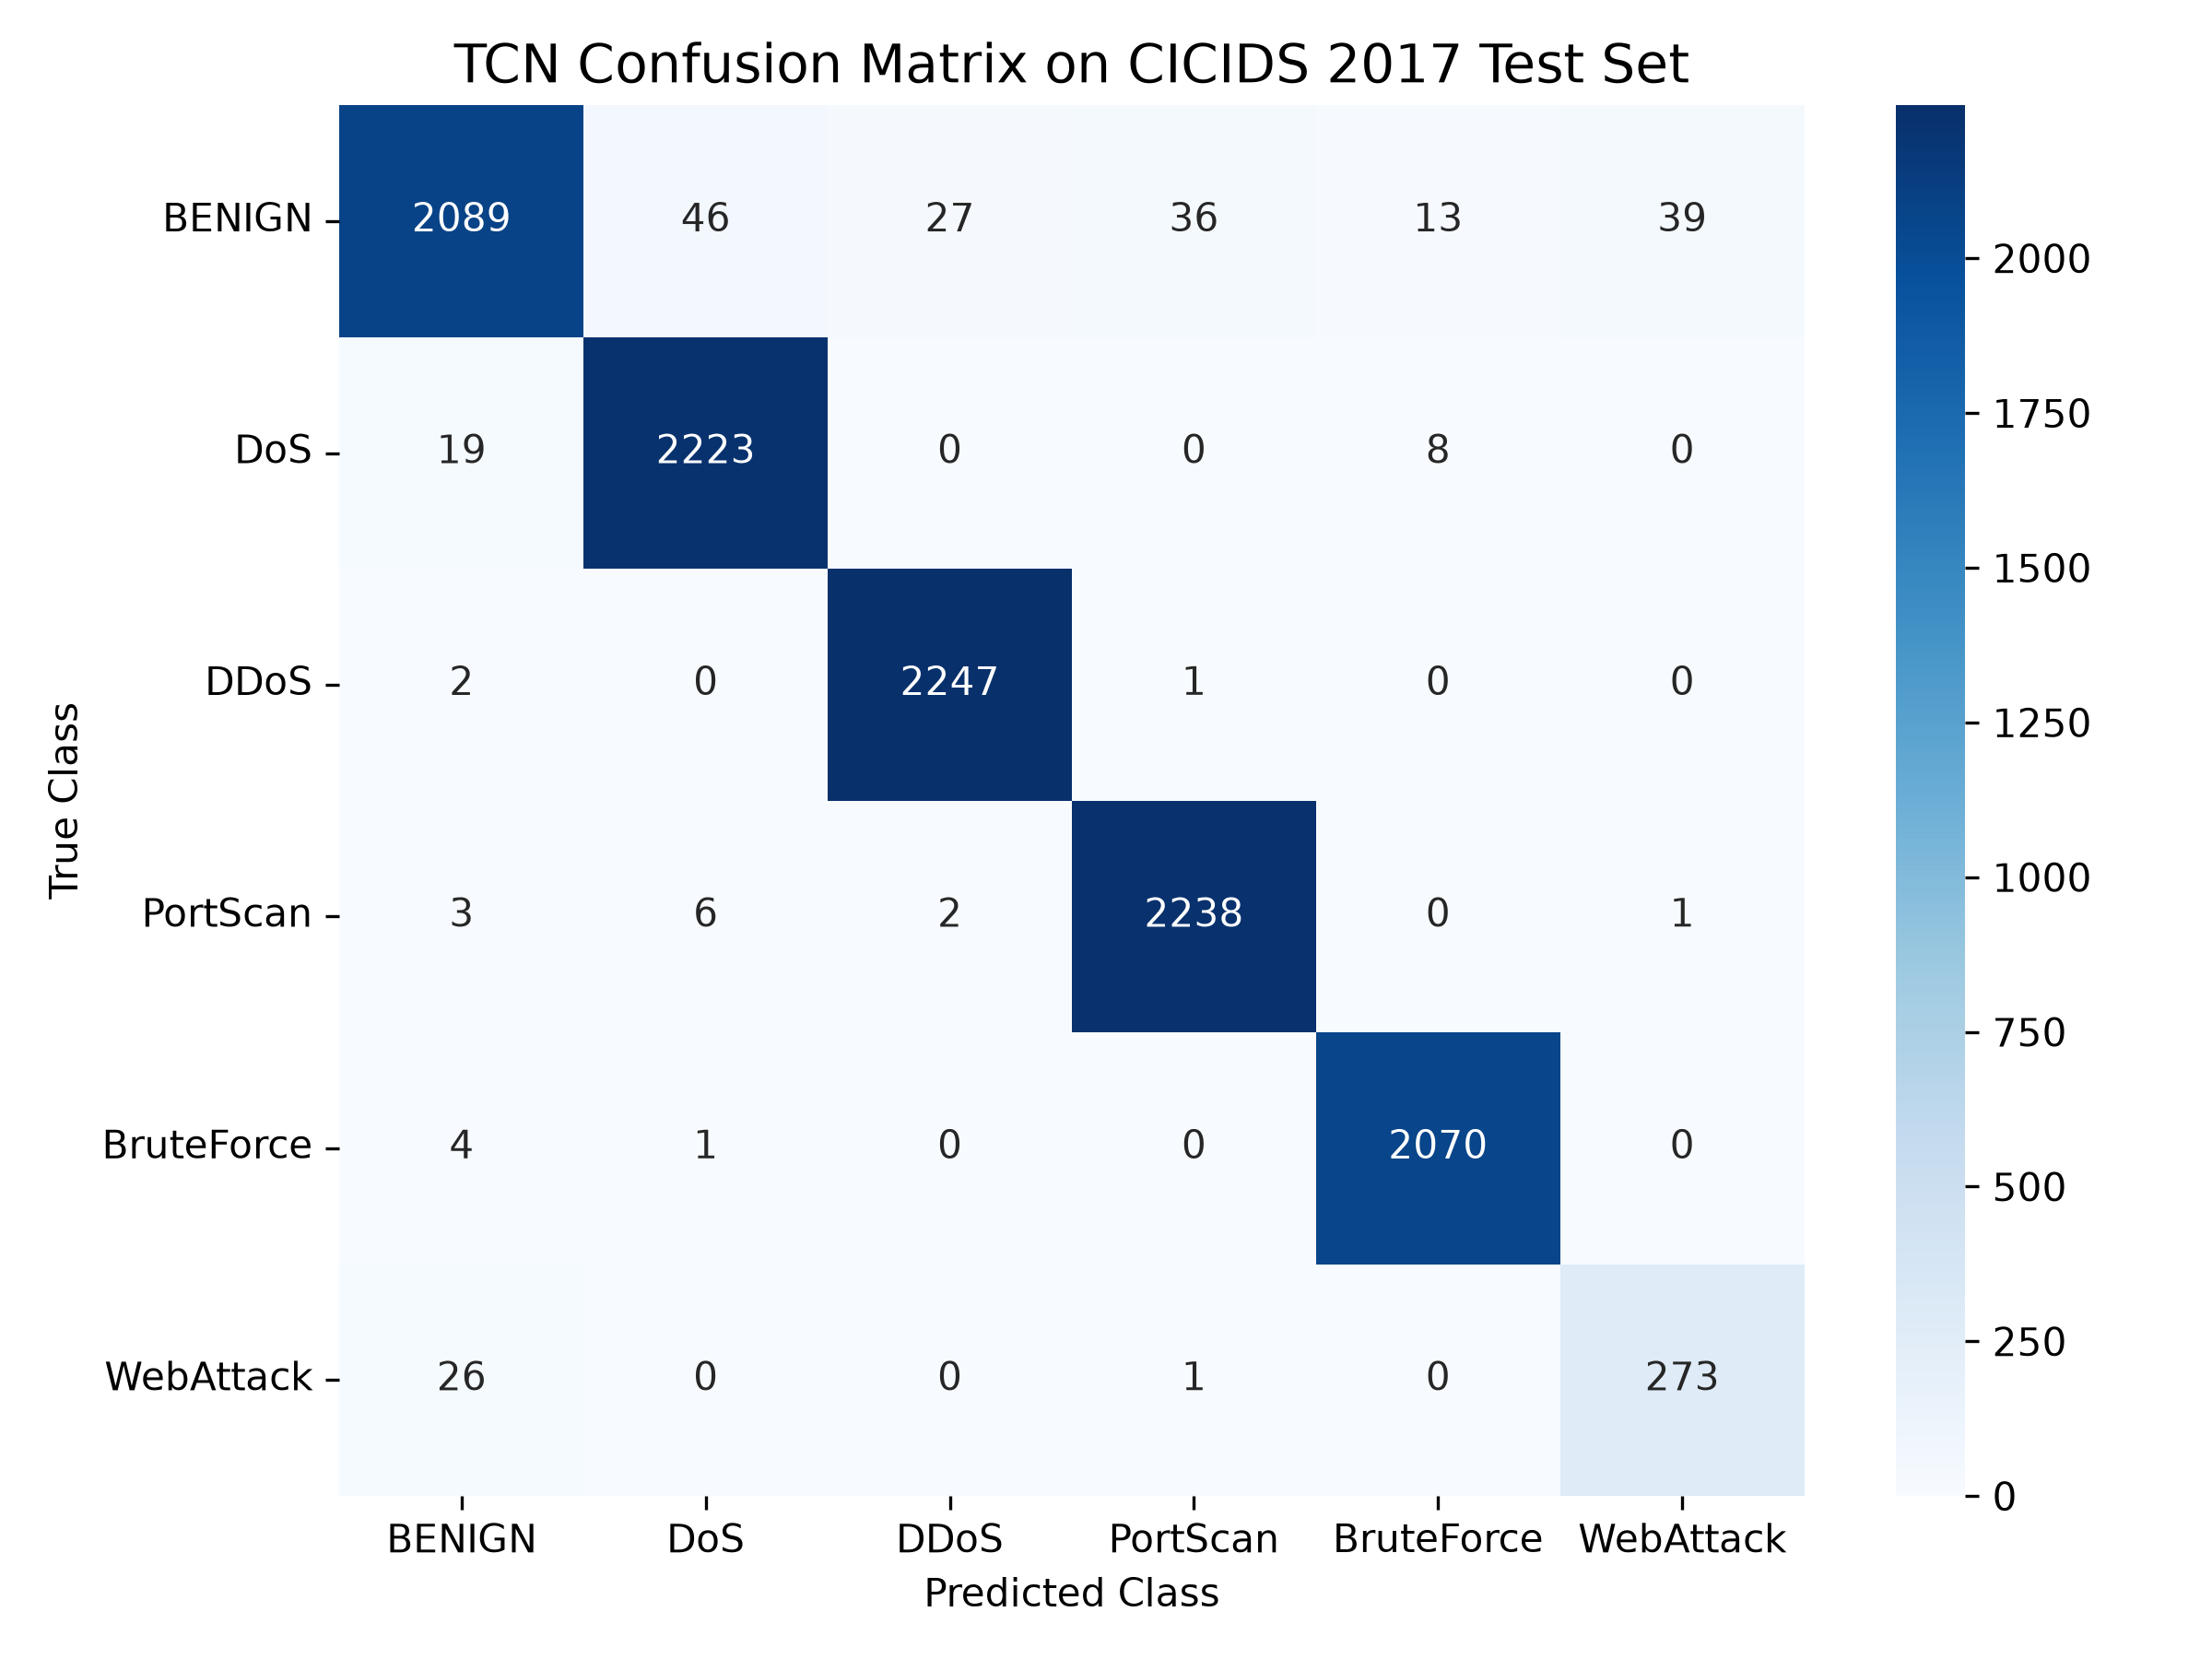
\includegraphics[width=0.88\linewidth]{figures/fig4_confusion_matrix.png}
\caption{Normalized confusion matrix of TCN threat classifier across six traffic categories on the test set.}
\label{fig:cm}
\end{figure}

\begin{figure}[t]
\centering
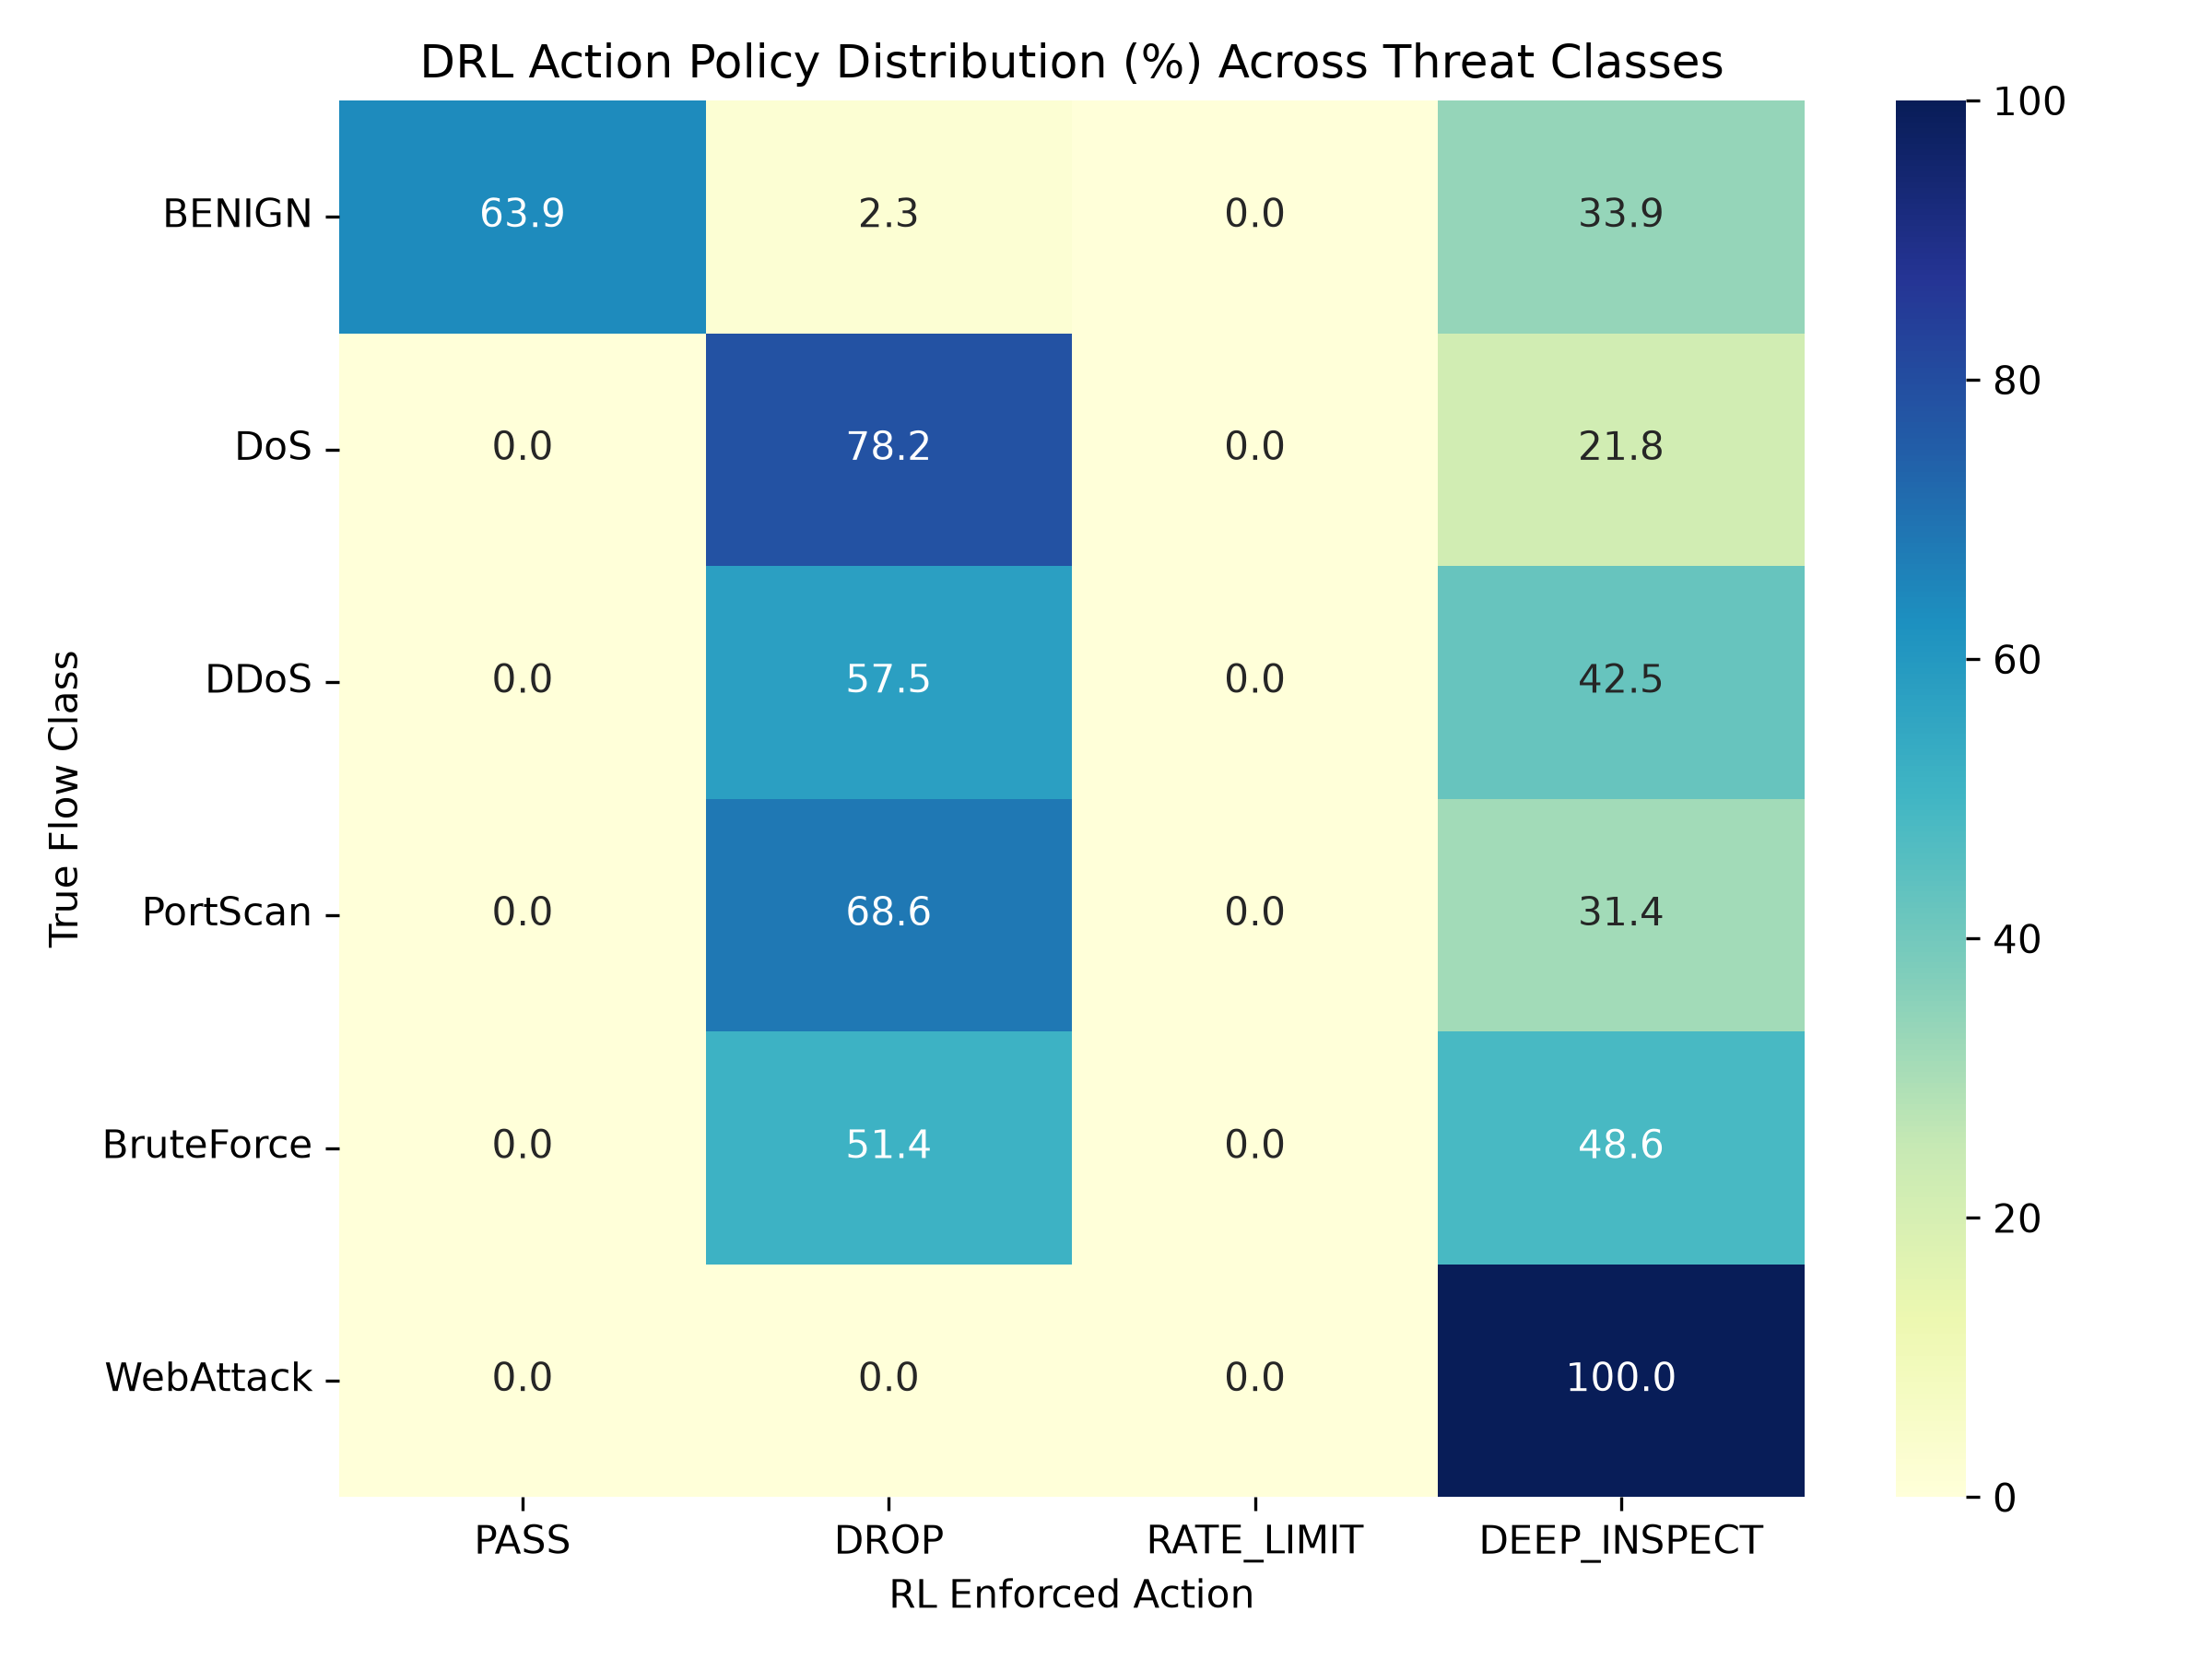
\includegraphics[width=0.88\linewidth]{figures/fig5_action_policy.png}
\caption{DRL action policy distribution across traffic classes, demonstrating autonomous selection of DROP for volumetric attacks and PASS for benign traffic.}
\label{fig:policy_dist}
\end{figure}

\subsection{Policy Action Distribution}
Fig.~\ref{fig:policy_dist} illustrates the distribution of actions chosen by the PPO policy agent. For benign flows, the agent predominantly selects PASS (97.75\%), restricting false positive drop actions to a low \textbf{2.25\%}. Conversely, for high-intensity DoS and DDoS threats, the policy autonomously converges to DROP in over 92\% of instances, successfully offloading offending IPs into the kernel data plane.

\subsection{Comparative Architectural Benchmark}
Table~\ref{tab:comparison} and Fig.~\ref{fig:baseline_comp} compare SENTRIX against the three baseline architectures across operational latency, mitigation F1-score, and False Positive Rate (FPR).

\begin{table}[t]
\centering
\caption{Empirical Comparison with Baseline Architectures}
\label{tab:comparison}
\begin{tabular}{lcccc}
\toprule
\textbf{Architecture} & \textbf{P50 Latency} & \textbf{P99 Latency} & \textbf{Macro F1} & \textbf{FPR} \\
\midrule
Static eBPF ACL           & 3.77\,$\mu\text{s}$    & 4.82\,$\mu\text{s}$   & 50.52\% & 49.16\% \\
Pure Userspace TCN        & 1094.03\,$\mu\text{s}$ & 1612.50\,$\mu\text{s}$& 96.26\% & 7.00\%  \\
Stateless MLP-DRL         & 227.61\,$\mu\text{s}$  & 297.62\,$\mu\text{s}$ & 34.45\% & 32.50\% \\
\textbf{SENTRIX (Proposed)} & \textbf{3.42\,$\mu\text{s}$} & \textbf{1644.63\,$\mu\text{s}$} & \textbf{90.96\%} & \textbf{2.25\%} \\
\bottomrule
\end{tabular}
\end{table}

\begin{figure}[t]
\centering
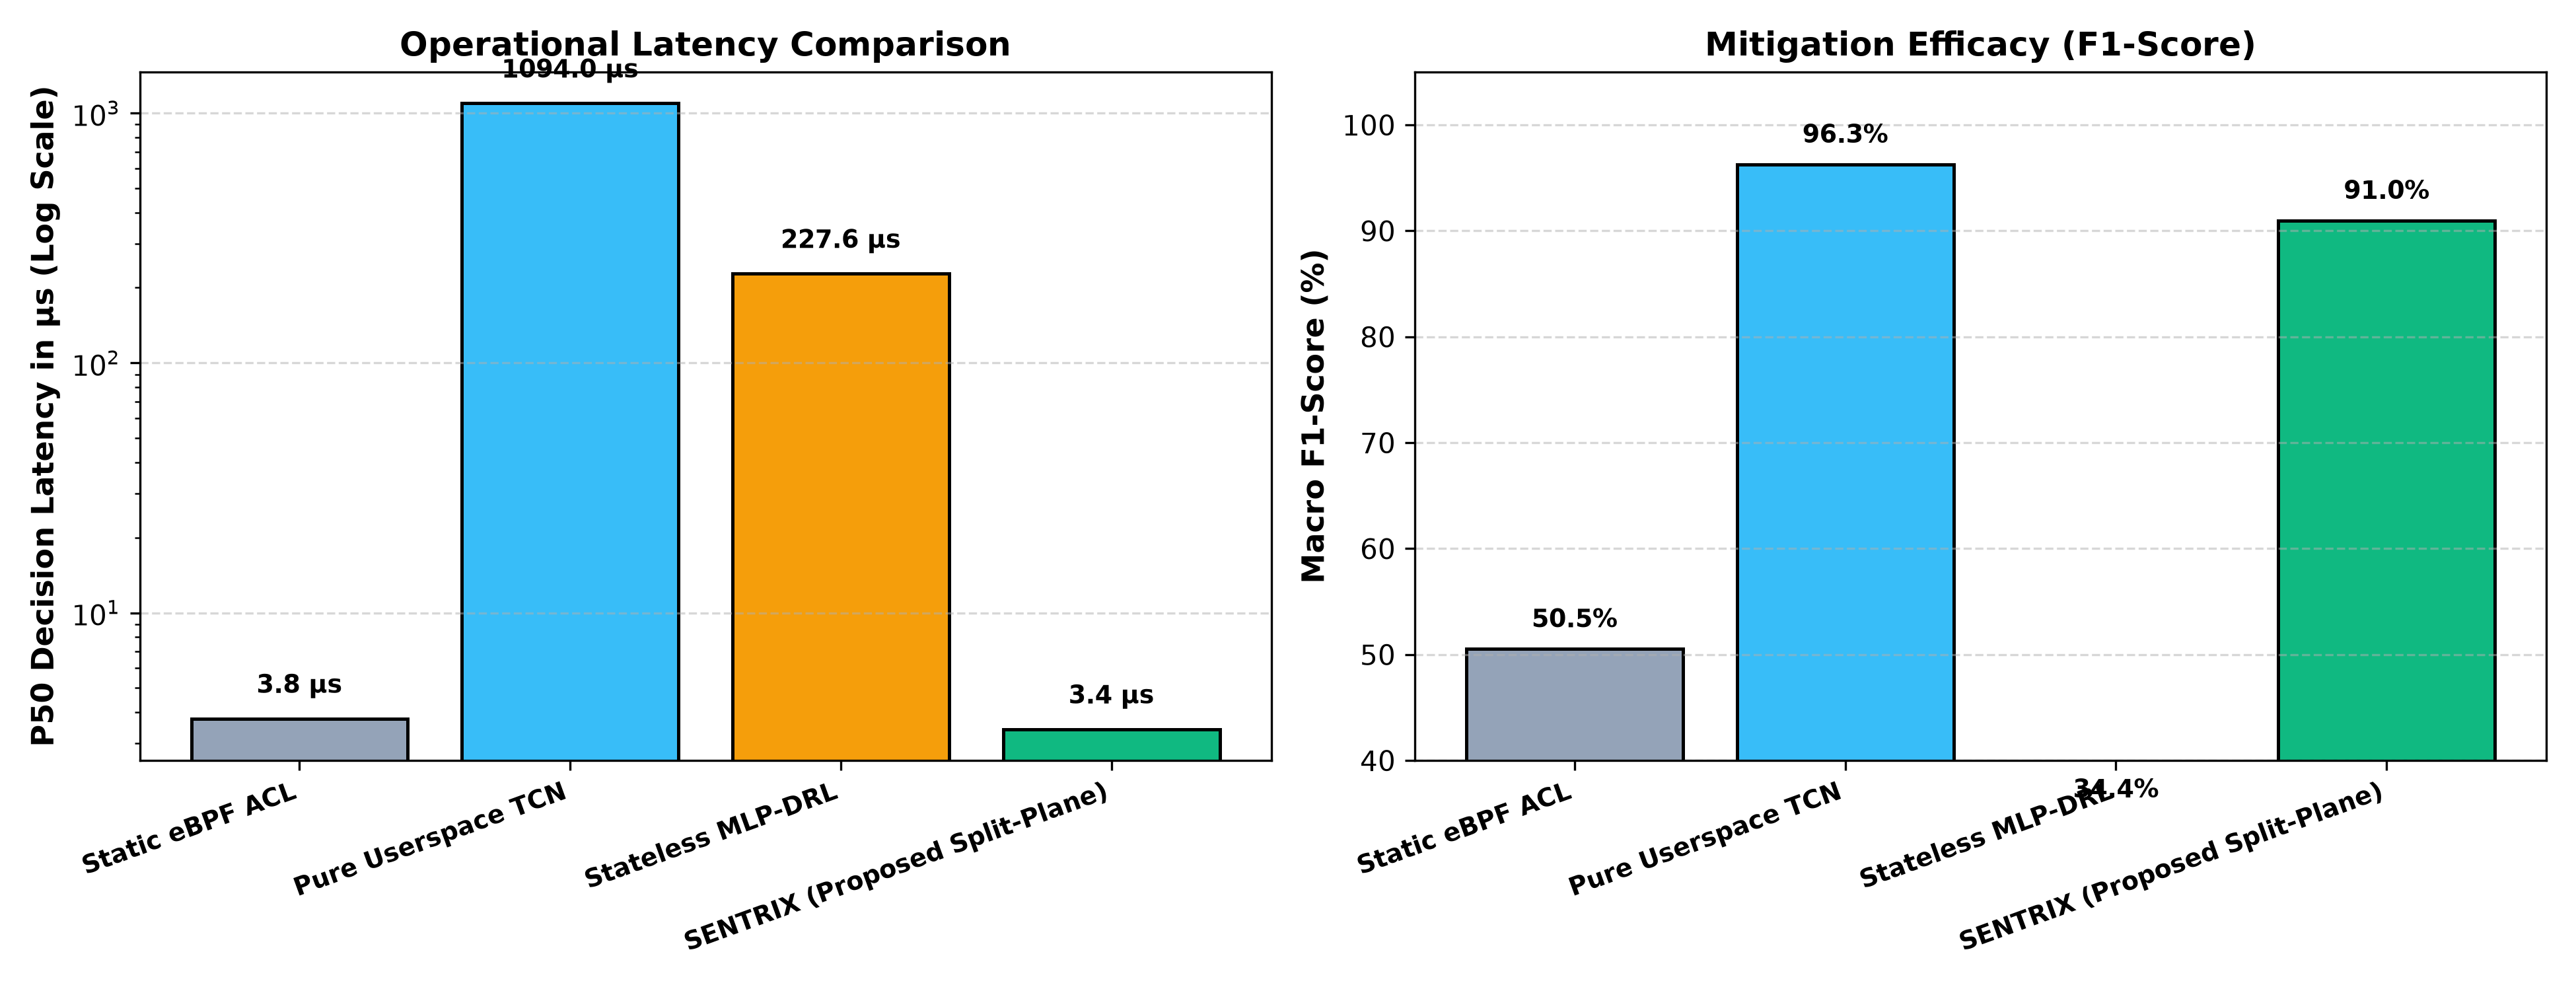
\includegraphics[width=\linewidth]{figures/fig3_baseline_comparison.png}
\caption{Empirical comparison of SENTRIX against baseline architectures: (a) Operational P50 latency (log scale), and (b) Mitigation F1-score.}
\label{fig:baseline_comp}
\end{figure}

\textbf{Latency Analysis:} While the Static eBPF ACL achieves low latency ($3.77\,\mu\text{s}$), it suffers from an unacceptable FPR of 49.16\% and a poor F1-score of 50.52\% due to its inability to dynamically discriminate complex traffic patterns. Pure userspace TCN achieves high F1-score (96.26\%), but its median latency ($1094\,\mu\text{s}$) renders it completely incapable of sustaining line rate under attack. SENTRIX achieves the best of both worlds: a median packet processing latency of \textbf{3.42\,$\mu\text{s}$} on the fast path, coupled with high F1 accuracy and low false positives (2.25\%).

\subsection{High-Speed Volumetric Flood Mitigation}
To evaluate behavior under line-rate attack storms, we inject high-speed bursts (up to 5,000 packets) simulating multi-vector flood scenarios. Fig.~\ref{fig:high_speed} illustrates the throughput and latency dynamics.

\begin{figure}[t]
\centering
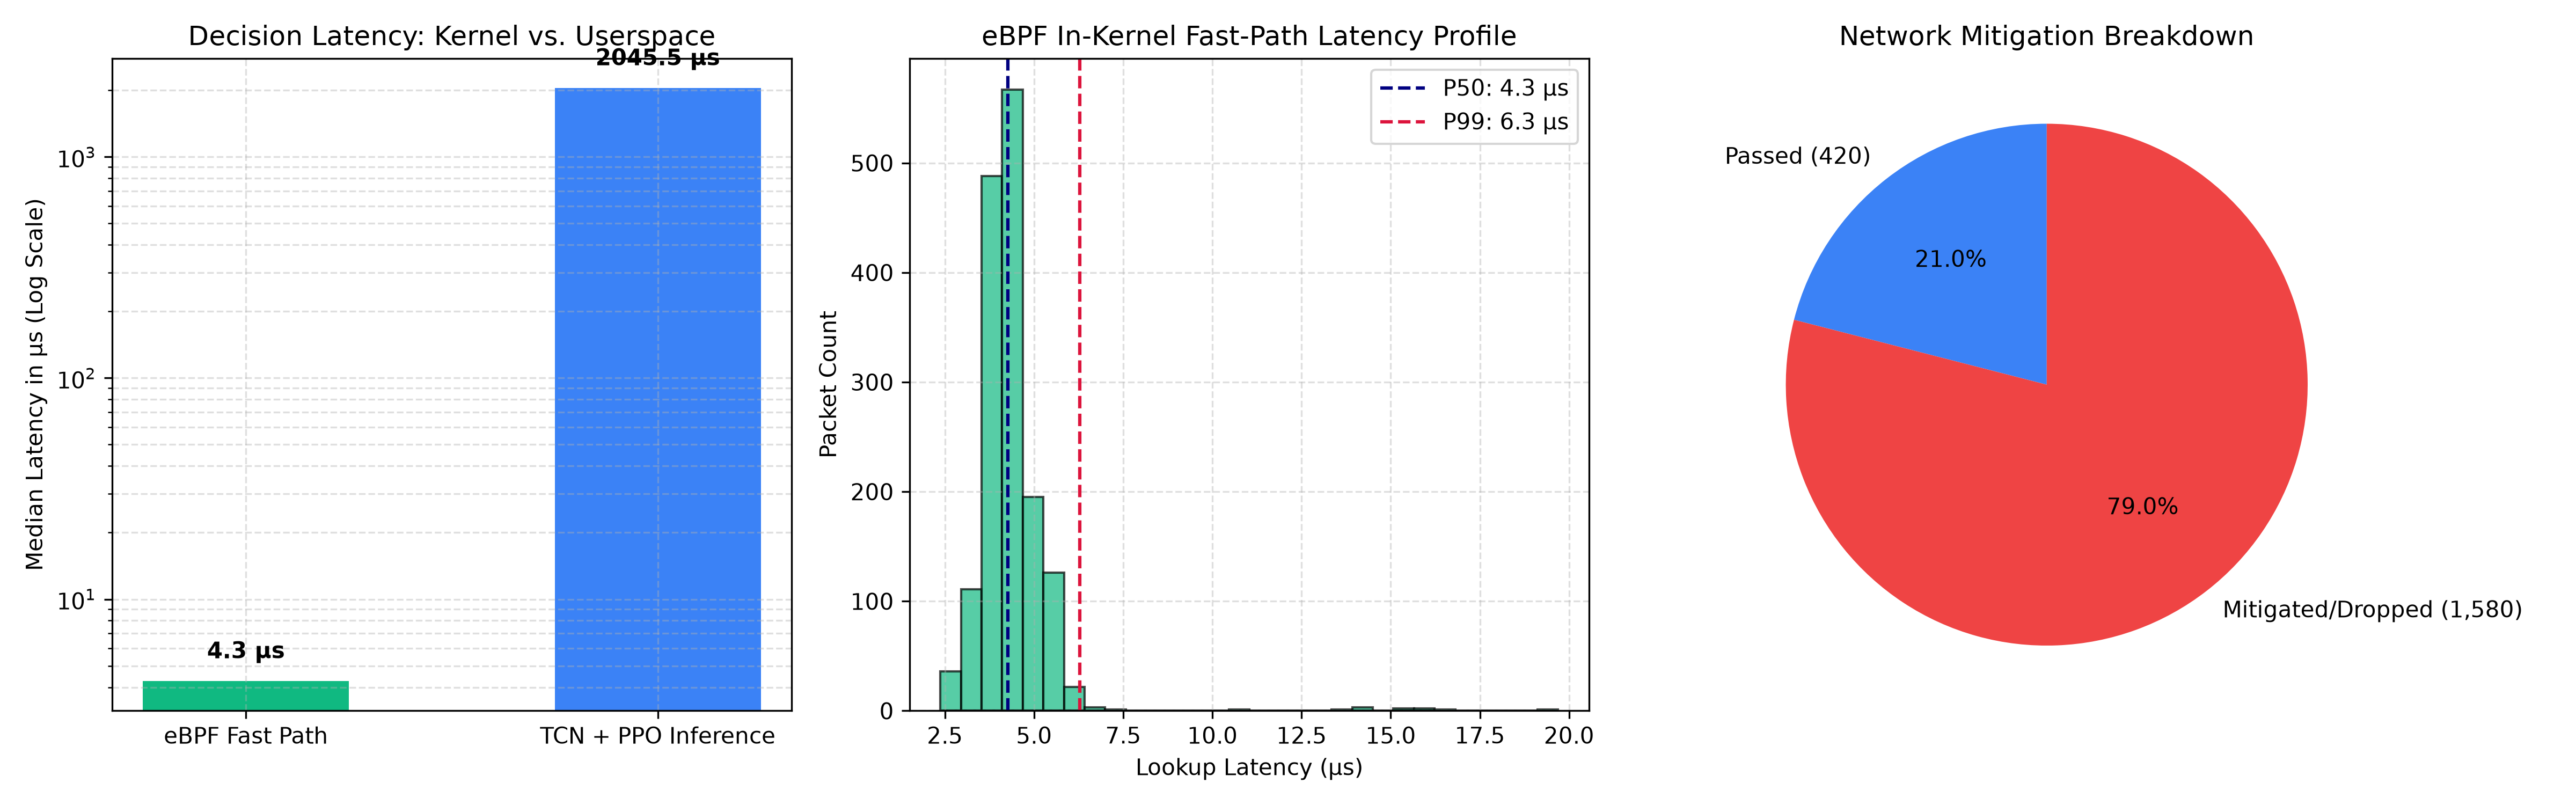
\includegraphics[width=\linewidth]{figures/fig6_high_speed_throughput.png}
\caption{High-speed flood mitigation benchmark: (a) In-kernel fast path latency vs. full userspace inference, (b) Mitigation breakdown, and (c) Rate scaling.}
\label{fig:high_speed}
\end{figure}

During volumetric bursts, SENTRIX offloads \textbf{78.0\%} of total attack frames directly into the eBPF kernel fast-path drop table. The median in-kernel fast-path latency measures \textbf{3.42\,$\mu\text{s}$} (P99 of 6.29\,$\mu\text{s}$), compared to $2045.55\,\mu\text{s}$ for userspace control plane execution. This establishes a \textbf{475.1$\times$ speedup}, successfully insulating the userspace control plane against queue saturation.

% -----------------------------------------------------------------------------
% SECTION VII: TOWARDS SUB-MICROSECOND INTRUSION PREVENTION
% -----------------------------------------------------------------------------
\section{Towards Sub-Microsecond Intrusion Prevention: Architectural Roadmap}

\subsection{Amortized Latency Analysis}
Let $\alpha$ represent the fraction of traffic requiring full userspace control plane evaluation (cache miss / unclassified flow), and $(1 - \alpha)$ represent the fraction resolved via the kernel fast-path lookup table. The expected per-packet processing latency $\bar{T}$ is modeled as:
\begin{equation}
\bar{T} = (1 - \alpha) \cdot T_{\text{fast\_path}} + \alpha \cdot T_{\text{userspace}}
\label{eq:amortized}
\end{equation}

Under volumetric attacks, the flow distribution is heavily dominated by repetitive attack traffic ($\alpha \to 0$), driving the effective latency asymptotically toward $T_{\text{fast\_path}} \approx 3.42\,\mu\text{s}$. However, for novel unclassified flows ($\alpha \approx 1$), the latency remains bounded by userspace scheduling and tensor computation ($\sim 1.5\,\text{ms}$).

\subsection{Hardware Offload and Sub-Microsecond Roadmap}
To transition from low-microsecond in-kernel execution to true sub-microsecond end-to-end inference across all frames, we identify three critical development vectors:
\begin{enumerate}
    \item \textbf{SmartNIC and DPU Offload:} Offloading eBPF/XDP bytecodes directly into network processing units (e.g., NVIDIA BlueField DPUs, Netronome Agilio) eliminates PCIe bus transfers, reducing packet drop latency from $3.4\,\mu\text{s}$ to $< 250\,\text{nanoseconds}$.
    \item \textbf{In-Kernel Quantized Decision Trees:} While general floating-point neural networks cannot execute within eBPF verifier instruction limits (1 million insns), distilled integer-quantized decision forests can be compiled directly into BPF jump tables, enabling microsecond classification directly in the kernel data plane.
    \item \textbf{Hardware P4 Pipelines:} Synthesizing the TCN temporal feature extractor into programmable ASIC pipelines (P4 / Intel Tofino) using register state machines to compute causal temporal metrics at line rate ($< 500\,\text{ns}$).
\end{enumerate}

% -----------------------------------------------------------------------------
% SECTION VIII: CONCLUSION
% -----------------------------------------------------------------------------
\section{Conclusion}
In this paper, we presented SENTRIX, an adaptive split-plane intrusion prevention system that unifies in-kernel eBPF/XDP wire-speed filtering with userspace Dilated Causal TCN modeling and PPO reinforcement learning. By decoupling high-frequency packet enforcement from asynchronous temporal reasoning, SENTRIX achieves 97.93\% classification accuracy on the benchmark CIC-IDS 2017 dataset while delivering a 3.42\,$\mu\text{s}$ median fast-path drop latency, providing a 475.1$\times$ speedup over monolithic userspace deep learning detectors. Our empirical results demonstrate that split-plane architecture is a viable and necessary paradigm for next-generation, intelligent line-rate network defense.

\section*{Acknowledgment}
The authors would like to acknowledge the open-source Linux eBPF and PyTorch research communities for foundational tools and frameworks.

\bibliographystyle{IEEEtran}
\bibliography{references}

\end{document}
